\begin{frame}
    \frametitle{Visualizzare ed Elaborare documenti XML}
    \addtocounter{nframe}{1}

     \begin{block}{XML Slyle Sheet Transformation: Modularità}
        \begin{itemize}
            \item XSLT consente di importare ed includere fogli XSLT dentro altri documenti XSLT
            \item mediante gli elementi \texttt{<xsl:import>} ed \texttt{<xsl:include>} 
        \end{itemize}
     \end{block}

\end{frame}

\begin{frame}
    \frametitle{Visualizzare ed Elaborare documenti XML}
    \addtocounter{nframe}{1}

     \begin{block}{XML Slyle Sheet Transformation}
        \begin{itemize}
            \item \textbf{inclusione}: le regole definite nel documento incluso hanno la stessa priorità delle regole definite nel documento XSLT principale.
            \item \textbf{importazione}: le regole definite nel documento principale hanno una priorità maggiore.
        \end{itemize}

     \end{block}

\end{frame}


\begin{frame}
    \frametitle{Visualizzare ed Elaborare documenti XML}
    \addtocounter{nframe}{1}
    
    \textbf{Dichiarazione XSD dell'elemento xsl:include}

    \begin{center}
        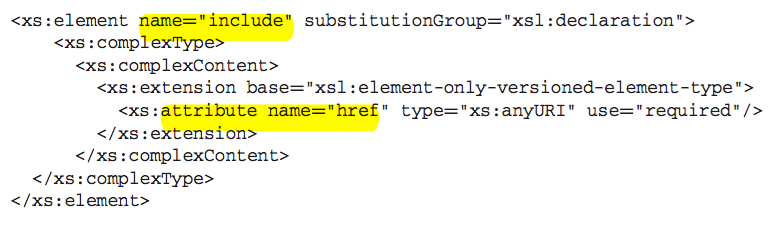
\includegraphics[width=.95\textwidth]{imgs/elementXSL-Include.png}
    \end{center}

\end{frame}

\begin{frame}
    \frametitle{Visualizzare ed Elaborare documenti XML}
    \addtocounter{nframe}{1}
    

     \begin{block}{XML Slyle Sheet Transformation: xsl:include}
        Dato un foglio esterno \texttt{esterno.xsl} per includerlo nel foglio principale si usa l'elemento: \\\texttt{<xsl:include href="esterno.xsl"/>}
     \end{block}

\end{frame}

\begin{frame}
    \frametitle{Visualizzare ed Elaborare documenti XML}
    \addtocounter{nframe}{1}
    
    \textbf{Dichiarazione XSD dell'elemento xsl:import}

    \begin{center}
        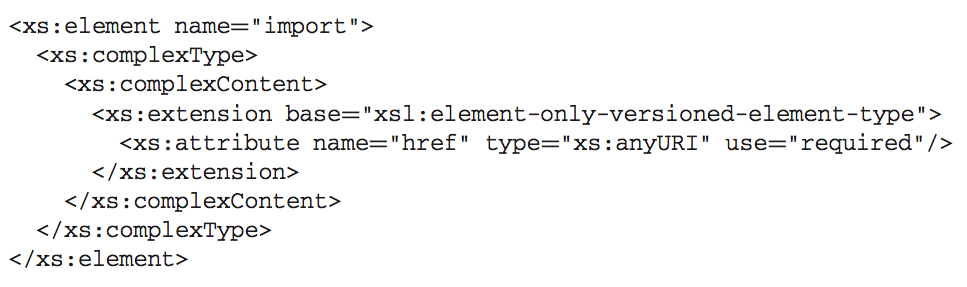
\includegraphics[width=.95\textwidth]{imgs/elementXSL-Import.png}
    \end{center}

\end{frame}

\begin{frame}
    \frametitle{Visualizzare ed Elaborare documenti XML}
    \addtocounter{nframe}{1}
    
    %\begin{center}
    %    
\includegraphics[width=.2\textwidth]{../imgs/tei-r.pdf}
    %\end{center}
    %\textit{In parte già disponibili nei moduli TEI di base}

     \begin{block}{XML Slyle Sheet Transformation: xsl:import}
        \texttt{<xsl:import href="esterno.xsl"/>}
        \\\texttt{<xsl:template match="/" >}
        \\\texttt{ <xsl:apply-imports/>}
        \\\texttt{</xsl:template>}
     \end{block}

\end{frame}

\begin{frame}
    \frametitle{Visualizzare ed Elaborare documenti XML}
    \addtocounter{nframe}{1}
    
    %\begin{center}
    %    
\includegraphics[width=.2\textwidth]{../imgs/tei-r.pdf}
    %\end{center}
    %\textit{In parte già disponibili nei moduli TEI di base}

     \begin{block}{XML Slyle Sheet Transformation: documenti multipli}
        \begin{itemize}
            \item Accedere ai nodi di un documento XML esterno a quello che si sta elaborando
            \item Utilizzando la funzionalità \texttt{document()}
        \end{itemize}

     \end{block}

     \begin{block}{XML Slyle Sheet Transformation: documenti multipli}
        \texttt{<xsl:value-of}
        \\\texttt{ select="document(’altro.xml’)/TEI/text/@type"}
        \\\texttt{/>}

     \end{block}

\end{frame}

\begin{frame}
    \frametitle{Visualizzare ed Elaborare documenti XML}
    \addtocounter{nframe}{1}
    
    %\begin{center}
    %    
\includegraphics[width=.2\textwidth]{../imgs/tei-r.pdf}
    %\end{center}
    %\textit{In parte già disponibili nei moduli TEI di base}

     \begin{block}{XML Slyle Sheet Transformation: XSLT 2.0}
        La \textit{recommendation} W3C per XSLT 2.0 è stata pubblicata nel 2007
     \end{block}

     \begin{block}{XML Slyle Sheet Transformation: documenti multipli}
       
        \texttt{<xsl:stylesheet} 
            \\\texttt{xmlns:xsl="http://www.w3.org/1999/XSL/Transform"} 
            \\\texttt{version="2.0" >}


     \end{block}

\end{frame}


\begin{frame}
    \frametitle{Visualizzare ed Elaborare documenti XML}
    \addtocounter{nframe}{1}
    

     \begin{block}{XML Slyle Sheet Transformation: XSLT 2.0}
        XSLT 2.0 permette di creare un documento di output in vari formati (xml, html, xhtml, text).
     \end{block}

\end{frame}

\begin{frame}
    \frametitle{Visualizzare ed Elaborare documenti XML}
    \addtocounter{nframe}{1}
    

     \begin{block}{XML Slyle Sheet Transformation: documenti multipli}
       
        \texttt{<xsl:template match="/" >}
        \\\texttt{ <xsl:result-document method="html" href="output.html" >}
        \\\texttt{ <xsl:apply-templates/>}
        \\\texttt{ </xsl:result-document>}
        \\\texttt{</xsl:template>}
            
     \end{block}

\end{frame}

\begin{frame}
    \frametitle{Visualizzare ed Elaborare documenti XML}
    \addtocounter{nframe}{1}

     \begin{block}{XML Slyle Sheet Transformation: XSLT 2.0}
        XSLT 2.0 permette di creare anche documenti multipli.
     \end{block}

\end{frame}

\begin{frame}
    \frametitle{Visualizzare ed Elaborare documenti XML}
    \addtocounter{nframe}{1}

     \begin{block}{XML Slyle Sheet Transformation: XSLT 2.0 esempio}
        \texttt{<template match="//div/[@type='book']" >}
        \\\texttt{<xsl:for-each select="div/[@type='chapter']" >}
        \\\texttt{<xsl:result-document}
           \\\texttt{method="html"}
           \\\texttt{href="\{@n\}.html" >}
           \\\texttt{<xsl:apply-templates/>}
        \\\texttt{</xsl:result-document>}
        \\\texttt{</xsl:for-each>}
        \\\texttt{</xsl:template>}
    
    \end{block}

\end{frame}

\begin{frame}
    \frametitle{Visualizzare ed Elaborare documenti XML}
    \addtocounter{nframe}{1}
    
    %\begin{center}
    %    
\includegraphics[width=.2\textwidth]{../imgs/tei-r.pdf}
    %\end{center}
    %\textit{In parte già disponibili nei moduli TEI di base}

     \begin{block}{XML Slyle Sheet Transformation: XSLT 2.0}
        \begin{itemize}
            \item elemento \texttt{<xsl:for-each-group>}: permette di selezionare un set di items
            \item processare un gruppo per volta
        \end{itemize}
        
     \end{block}

\end{frame}

\begin{frame}
    \frametitle{Visualizzare ed Elaborare documenti XML}
    \addtocounter{nframe}{1}
    
     \begin{block}{XML Slyle Sheet Transformation: XSLT 2.0}
        \textit{Possibili attributi}
        \begin{itemize}
            \item group-by
            \item group-adjacent
            \item group-starting-with
            \item group-ending-with
        \end{itemize}
    
    \end{block}

\end{frame}

\begin{frame}
    \frametitle{Visualizzare ed Elaborare documenti XML}
    \addtocounter{nframe}{1}
    
        \textit{Esempio elemento for-each-group}

    \begin{center}
        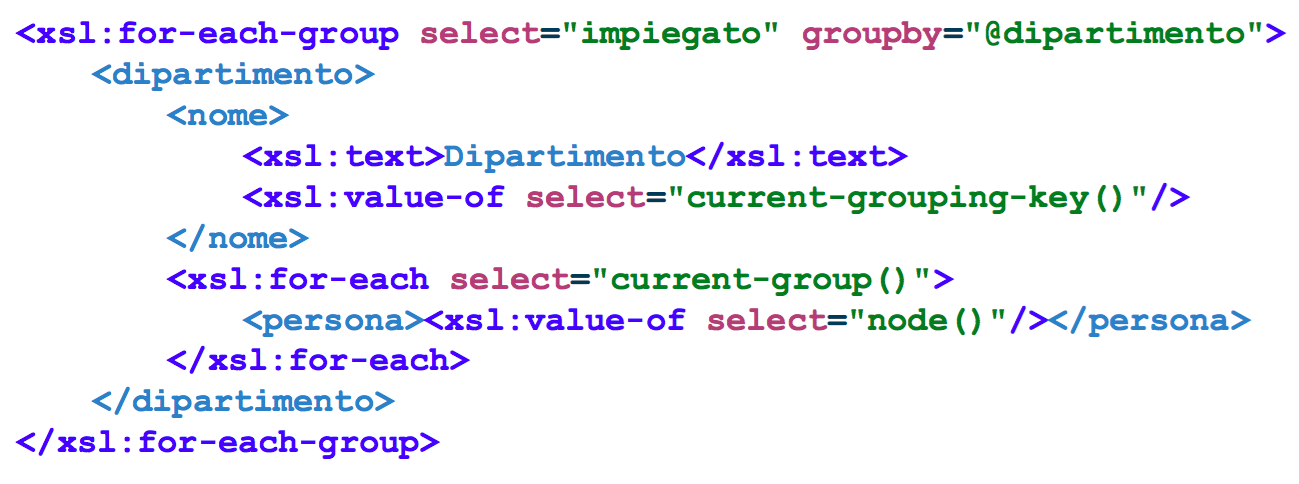
\includegraphics[width=.95\textwidth]{imgs/esempio-groupBy.png}
    \end{center}

\end{frame}

\begin{frame}
    \frametitle{Visualizzare ed Elaborare documenti XML}
    \addtocounter{nframe}{1}
    
        \textit{Espressioni condizionali if()}

    \begin{center}
        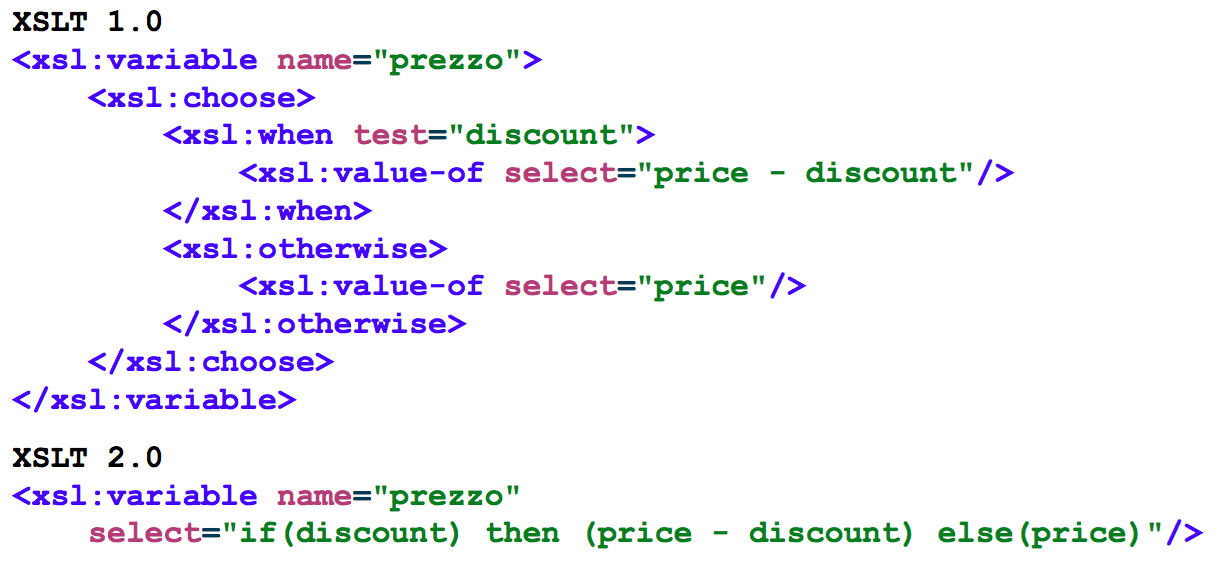
\includegraphics[width=.95\textwidth]{imgs/esempio-espressioneCondizionale.png}
    \end{center}

\end{frame}



